\let\negmedspace\undefined
\let\negthickspace\undefined
\documentclass[journal]{IEEEtran}
\usepackage[a5paper, margin=10mm, onecolumn]{geometry}
\usepackage{lmodern} % Ensure lmodern is loaded for pdflatex
\usepackage{tfrupee} % Include tfrupee package

\setlength{\headheight}{1cm} % Set the height of the header box
\setlength{\headsep}{0mm}     % Set the distance between the header box and the top of the text

\usepackage{gvv-book}
\usepackage{gvv}
\usepackage{cite}
\usepackage{amsmath,amssymb,amsfonts,amsthm}
\usepackage{algorithmic}
\usepackage{graphicx}
\usepackage{textcomp}
\usepackage{xcolor}
\usepackage{txfonts}
\usepackage{listings}
\usepackage{enumitem}
\usepackage{mathtools}
\usepackage{gensymb}
\usepackage{comment}
\usepackage[breaklinks=true]{hyperref}
\usepackage{tkz-euclide} 
\usepackage{listings}
\usepackage{gvv}                                        
\def\inputGnumericTable{}                                 
\usepackage[latin1]{inputenc}                                
\usepackage{color}                                            
\usepackage{array}                                            
\usepackage{longtable}                                       
\usepackage{calc}                                             
\usepackage{multirow}                                         
\usepackage{hhline}                                           
\usepackage{ifthen}                                           
\usepackage{lscape}
\usepackage{tikz}
\usepackage{tcolorbox}
\usetikzlibrary{matrix}
\usepackage{url}
\usepackage{xcolor}\begin{document}

\bibliographystyle{IEEEtran}
\vspace{3cm}

\title{10.3.5.4.3}
\author{EE24BTECH11018 - Durgi Swaraj Sharma}
% \maketitle
% \newpage
% \bigskip
{\let\newpage\relax\maketitle}
\textbf{Question:}
Yash scored $40$ marks in a test, getting $3$ marks for each right answer and losing $1$ mark for each wrong answer. Had $4$ marks been awarded for each correct answer and $2$ marks been deducted for each incorrect answer, then Yash would have scored $50$ marks. How many questions were there in the test?

\solution 

Writing the problem in mathematical equations,
\begin{align}
  3x-1y&=40\\
  4x-2y&=50\\
  x+y&=?
\end{align}
where $x$ represents the number of correct answers, $y$ represents the number of incorrect answers. $x+y$ gives us the total number of questions in the test. 

Representing using matrices,
\begin{align}
    \myvec{
        3 & -1\\
        4 & -2
    } \myvec{x \\ y}= \myvec{ 40 \\ 50}
\end{align}
\textbf{LU Decomposition}\\
We shall solve this system of equations by LU Decomposition. Any non-sigular matrix can be represented as a product of a lower triangular matrix $L$ and an upper triangular matrix $U$
\begin{align}
    A\vec{x} = LU\vec{x} = \vec{b}
\end{align}
Applying row reduction on $A$ to find $U$,
\begin{align}
  \myvec{3 & -1\\ 4 & -2} \xrightarrow{R_2 \leftrightarrow R_2 - \frac{4}{3}R_1} \myvec{3 & -1 \\ 0 & -\frac{2}{3}}
\end{align}
Let 
\begin{align}
    L = \myvec{1 & 0\\ l_{21} & 1}
\end{align}
$l_{21}$ is the multiplier used to zero $a_{21}$, so $l_{21} = \frac{4}{3}$.\\
Now,
\begin{align}
  A = \myvec{3 & -1 \\ 4 & -2} = \myvec{1 & 0 \\ \frac{4}{3} & 1}\myvec{3 & -1 \\ 0 & -\frac{2}{3}}
\end{align}
We have thus obtained LU Decomposition of the matrix $A$. 

The LU Decomposition of matrix $A$ can also be obtained by Doolittle's Algorithm. This gives us update equations to construct the $L$ and $U$ matrix. \\
Elements of $U$ matrix:\\
For each column $j$,
\begin{align}
  U_{ij} = \begin{cases}
    A_{ij} & i=0 \\
    A_{ij} - \sum _{k=0}^{i-1} L_{ik}U_{kj} & i>0
  \end{cases}
\end{align}
Elements of $L$ matrix:\\
For each row $i$,
\begin{align}
  L_{ij} = \begin{cases}
    \frac{A_{ij}}{U_{ij}} & j=0 \\
    \frac{A_{ij} - \sum _{k=0}^{j-1} L_{ik}U_{kj}}{U_{ij}} & j>0
  \end{cases}
\end{align}
The above proccess decomposes any non-sigular matrix $A$ into an upper-triangular matrix $U$ and a lower-triangular matrix $L$.\\
Now, let
\begin{align}
  U\vec{x} = \vec{y}\\
  L\vec{y} = \vec{b}\label{1}
\end{align}
Substituting the values,
\begin{align}
  \myvec{1 & 0 \\ \frac{4}{3} & 1}\myvec{y_1 \\ y_2} &= \myvec{40 \\ 50}\\
  \myvec{y_1 \\ y_2} &= \myvec{40 \\ -\frac{10}{3}}
\end{align}
Backsubstituting,
\begin{align}
  \myvec{3 & -1 \\ 0 & -\frac{2}{3}}\myvec{x_1 \\ x_2} &= \myvec{40 \\ -\frac{10}{3}}\\
  \myvec{x_1 \\ x_2} &= \myvec{ 15 \\ 5}
\end{align}
Thus, the system of equations is solved at $\vec{x} = \myvec{15 \\ 5}$.
The total number of questions in the test is \textbf{20}.
\begin{figure}[h!]
   \centering
   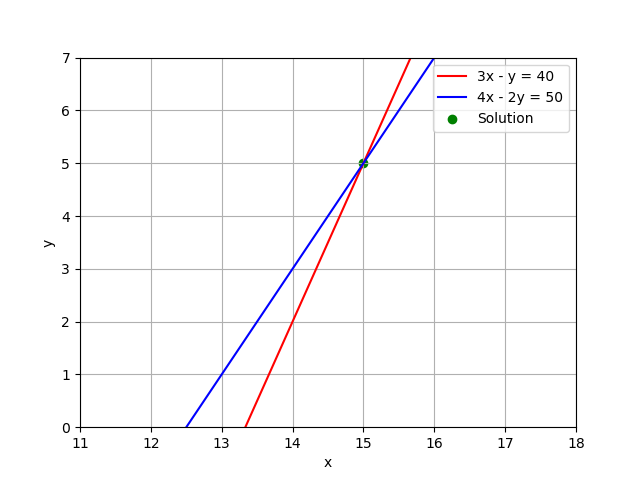
\includegraphics[width=\columnwidth]{/home/gvt1/sdcard/github/EE1003/Assignment5/figs/fig.png}
   \caption{Solving the system of equations, $3x - 1y = 40, 4x - 2y = 50$}
\end{figure}
\end{document}
